\section{Implementation details}
\label{app:impl}
\textbf{Scoring.} Every configuration is a chat (ChatML) or raw prompt; the model's next-token logits at the position after the answer prefix (``The answer is ('' or ``Answer:'') are restricted to the letters A--J that exist for the question, and the arg-max letter is the prediction. The shared prefix (system prompt and demonstrations) is computed once and its key/value cache re-used for all questions (verified to reproduce uncached logits up to fp16 storage rounding). fp32 inference on 4 CPU cores; no sampling.
\textbf{World A} ($K{=}40$): instruction $\in$ \{none (template default system prompt), ``You are a helpful assistant.'', ``Answer the following multiple-choice question. Respond with the letter of the correct option.'', ``You are a world-class expert across all academic disciplines. Choose the single best answer.'', ``Read the question carefully, eliminate options that are clearly wrong, and select the most likely correct answer.'', ``The following are multiple choice questions from a difficult university-level exam. Be precise.'', ``Be careful: many questions look easy but contain subtle traps. Think about what the question is really asking before choosing.'', ``Reply with only the letter of the best option.''\} $\times$ demonstration set $\in$ \{zero-shot, four random 3-shot sets from the 70 MMLU-Pro validation questions\}; demonstrations are answer-only chat turns.
\textbf{World B} ($K{=}40$): format $\in$ \{chat with ``Options:'' block and an instruction line; raw text (no chat template, ``Question: \dots Answer:''); chat with ``(A)''-style options and ``Answer:'' prefix; chat without the instruction line; chat with options before the question\} $\times$ demonstrations $\in$ \{zero-shot, 3 random, 3 validation questions that all have answer ``A'', 8 random\} $\times$ instruction $\in$ \{none, ``world-class expert''\}.
\textbf{Pool.} Questions whose ``question + options'' text has at most 200 Qwen tokens (about $7{,}900$ of $12{,}032$ test questions); a seeded permutation (seed 12345) and the first 750 (world D: 450) are used, with the same Qwen tokenizer defining the pool for every model. Category composition of the eligible set: math 15\%, physics 12\%, other 10\%, economics 9\%, health 8\%, \dots, law 2\%, history 2\%.
\textbf{Optimizers} (code: \texttt{code/sim\_lib.py}). \emph{Exhaustive}: all $K$ configurations on all $n$ questions. \emph{Random-8}: 8 random configurations. \emph{SH}: successive halving over questions, total budget $0.5Kn$ (config, question) evaluations, $\lceil\log_2 K\rceil$ rounds, final winner re-scored on all of $D$ for the report. \emph{Minibatch}: 30 trials; each proposes a uniformly random configuration (prob.\ 0.5) or a one-factor neighbour of the current best-by-running-mean, scores it on a random minibatch of $0.25n$ questions, and every 10 trials the incumbent is scored on all of $D$; the final choice is the best full-$D$ score. \emph{Greedy}: from a random start, up to 3 sweeps of coordinate ascent over the factor axes with full-$D$ scores. Ties are broken uniformly at random.
\textbf{Protocol details} (\texttt{code/sim\_lib.py}, \texttt{code/episodes.py}). Wilson intervals; holdout fractions $f\in\{0.3,0.5,0.7\}$; 5-fold cross-fit; replay bootstrap $B{=}100$; max-$t$ uses 1000 Gaussian multipliers and studentised errors with $\hat\sigma_k=\sqrt{\hat p_k(1-\hat p_k)}$ (floored at $1/(2\sqrt n)$); empirical Bayes: $\theta_k=g+d_k$, $d_k\sim N(0,\tau^2)$, centred paired covariance $\hat S/n$, $\hat\tau^2=\max\{0,\|\hat d\|^2/(m-1)-\mathrm{tr}(P\hat SP)/(m-1)\}$, posterior mean $\bar{\bar y}+\hat B\hat d_{\hat k}$ with $\hat B=\hat\tau^2/(\hat\tau^2+v_{\hat k})$; the reported interval is est.\ $\pm1.96\sqrt{u+v_{\hat k}}$ with $u$ the sampling variance of the grand mean (a ``posterior'' interval with $\hat B v_{\hat k}$ instead of $v_{\hat k}$ under-covers: 0.85--0.95 in our worlds); conditional inference: truncation limits from the polyhedron $\{\bar Y_k\ge\bar Y_j\,\forall j\}$ with the empirical covariance, exact ties replaced by a uniform jitter of width $1/n$; Ladder with step $\eta=n^{-1/2}$ ($n^{-1/3}$ variant also computed, deploys much worse configurations: $-7.0$ points in A$\cup$B at $n{=}100$). Max-$t$, empirical Bayes and conditional inference are applied to the set of fully evaluated configurations; for adaptive optimizers (greedy, minibatch) this is heuristic, and for SH it is undefined (one fully evaluated configuration).
\textbf{Synthetic worlds} (\texttt{code/worlds.py::synth\_world}): $Y_{ki}\sim\mathrm{Bernoulli}(\mathrm{sigmoid}(\mu+d_i+c_k+s\,e_{ki}))$ with $d_i\sim N(0,1.2^2)$ (difficulty), $c_k\sim N(0,\tau^2)$ (configuration effect), $e_{ki}\sim N(0,1)$ (interaction, controls $\rho$), $N=20000$; sweep $K\in\{2,5,10,40,160\}$, $\tau\in\{0,.05,.1,.2,.4\}$, $s\in\{.3,.8,1.5\}$, $n\in\{50,\dots,800\}$, 400 episodes per cell.

\section{Additional results}
\label{app:extra}
\begin{figure}[H]\centering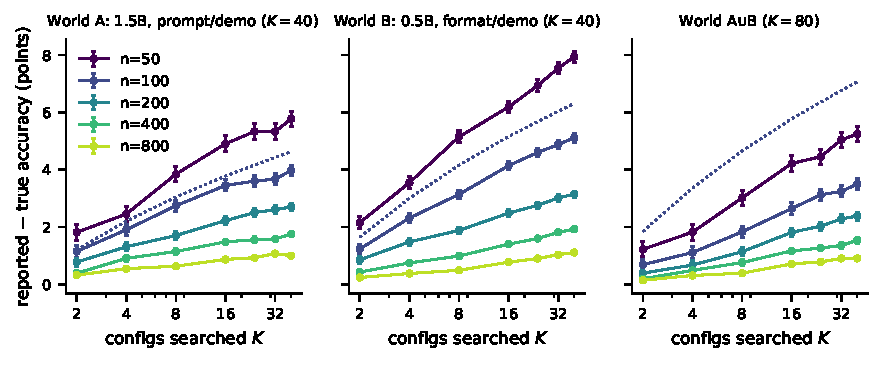
\includegraphics[width=.95\textwidth]{figs/gap_vs_K.pdf}
\caption{Optimism of exhaustive search over a random subset of $K$ of the configurations of each world, by dev-set size (95\% CI; 1000 episodes per point). Dotted ($n{=}100$): equal-quality prediction $\sigma_n\sqrt{1-\bar\rho}\,m_K$, an upper reference when configurations differ in quality.}\label{fig:ksweep}\end{figure}
\begin{figure}[H]\centering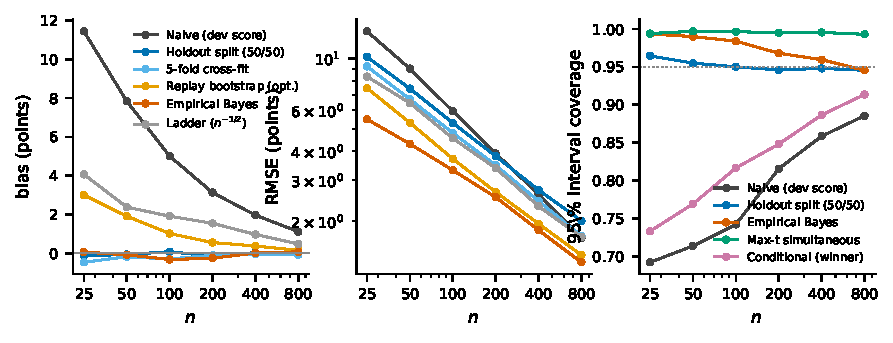
\includegraphics[width=.75\textwidth]{figs/protocols_b05.pdf}\\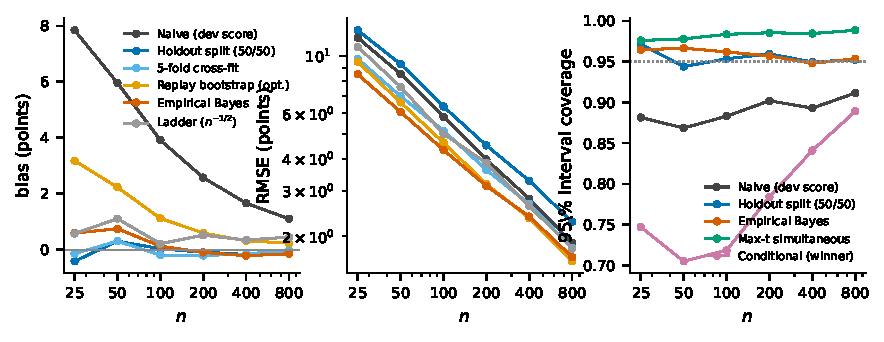
\includegraphics[width=.75\textwidth]{figs/protocols_q15.pdf}\\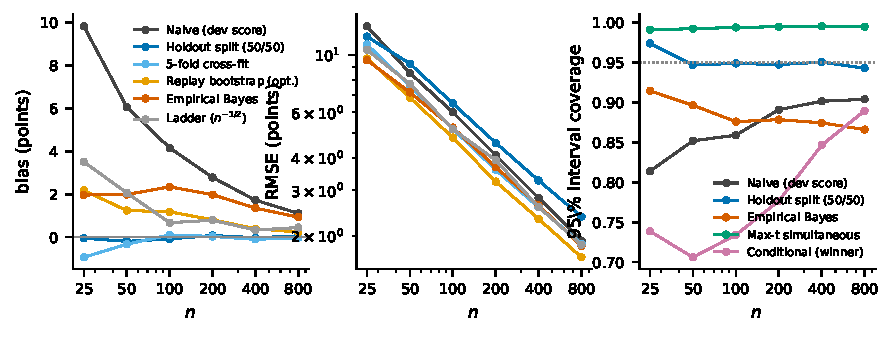
\includegraphics[width=.75\textwidth]{figs/protocols_mix.pdf}
\caption{Bias, RMSE and interval coverage of the protocols against $n$ for exhaustive search in world B (top), A (middle), A$\cup$B (bottom); worlds C and D: \cref{tab:proto_extra}.}\label{fig:protocols}\end{figure}
\begin{table}[H]
\caption{Protocols for every optimizer, $n{=}100$ (points; coverage as fraction). Bias and RMSE of the naive score; RMSE of the 50/50 holdout; bias and RMSE of the replay bootstrap; bias, RMSE and coverage of empirical Bayes (heuristic for greedy/minibatch, undefined for SH).}\label{tab:allopt}
\centering\scriptsize\setlength{\tabcolsep}{4pt}
\begin{tabular}{lrrrrrrrr}\toprule
\multicolumn{1}{l}{} & \multicolumn{2}{c}{naive} & hold. & \multicolumn{2}{c}{replay boot.} & \multicolumn{3}{c}{emp.\ Bayes} \\
 & bias & RMSE & RMSE & bias & RMSE & bias & RMSE & cov. \\\midrule
\multicolumn{9}{l}{\emph{A: Qwen2.5-1.5B, prompt/demo grid ($K{=}40$)}} \\
Exhaustive & 3.9 & 5.8 & 6.4 & 1.1 & 4.6 & 0.1 & 4.3 & 0.96 \\
Random-8 & 2.7 & 5.2 & 6.7 & 0.8 & 4.6 & 0.4 & 4.4 & 0.95 \\
Succ. halving & 3.4 & 5.6 & 6.7 & 0.9 & 4.6 & -- & -- & -- \\
Minibatch (MIPRO-like) & 1.7 & 4.9 & 6.5 & 0.3 & 4.6 & 0.8 & 4.3 & 0.97 \\
Greedy coord. & 3.5 & 5.7 & 6.5 & 1.1 & 4.8 & 1.0 & 4.7 & 0.95 \\
\multicolumn{9}{l}{\emph{B: Qwen2.5-0.5B, format/demo grid ($K{=}40$)}} \\
Exhaustive & 5.0 & 5.9 & 5.3 & 1.0 & 3.7 & -0.3 & 3.3 & 0.98 \\
Random-8 & 3.2 & 4.7 & 5.4 & 0.6 & 3.5 & -0.3 & 3.4 & 0.97 \\
Succ. halving & 4.6 & 5.7 & 5.3 & 1.0 & 3.7 & -- & -- & -- \\
Minibatch (MIPRO-like) & 3.0 & 4.7 & 5.2 & 0.4 & 3.7 & 1.4 & 3.6 & 0.99 \\
Greedy coord. & 4.4 & 5.5 & 5.3 & 1.1 & 3.7 & 1.0 & 3.6 & 0.96 \\
\multicolumn{9}{l}{\emph{A$\cup$B: union ($K{=}80$)}} \\
Exhaustive & 4.2 & 6.0 & 6.5 & 1.2 & 4.8 & 2.3 & 5.2 & 0.88 \\
Random-8 & 1.8 & 4.9 & 6.6 & 0.3 & 4.7 & 0.2 & 4.9 & 0.91 \\
Succ. halving & 3.4 & 5.6 & 6.6 & 0.6 & 4.6 & -- & -- & -- \\
Minibatch (MIPRO-like) & 1.7 & 4.9 & 6.6 & 0.2 & 4.8 & 0.9 & 4.7 & 0.97 \\
Greedy coord. & 3.7 & 5.5 & 6.4 & 1.0 & 4.3 & 2.0 & 4.8 & 0.92 \\
\bottomrule
\end{tabular}

\end{table}
\begin{table}[H]
\caption{Draws without replacement (dev set $D$ of $n$ distinct pool questions): optimism relative to the pool accuracy and relative to the accuracy on the \emph{remaining} pool questions (fresh), compared with the i.i.d.\ design of the main text (points).}\label{tab:norepl}
\centering\scriptsize\setlength{\tabcolsep}{4pt}
\begin{tabular}{lrrr}\toprule
 & i.i.d.\ (main) & w/o repl., vs pool & w/o repl., vs fresh \\\midrule
\multicolumn{4}{l}{\emph{A: Qwen2.5-1.5B, prompt/demo grid ($K{=}40$)}} \\
Exhaustive, $n{=}50$ & 6.0 & 5.7 & 6.1$\pm$0.3 \\
Exhaustive, $n{=}100$ & 3.9 & 3.6 & 4.2$\pm$0.2 \\
Exhaustive, $n{=}200$ & 2.6 & 2.4 & 3.3$\pm$0.2 \\
Minibatch (MIPRO-like), $n{=}50$ & 2.4 & 2.3 & 2.5$\pm$0.3 \\
Minibatch (MIPRO-like), $n{=}100$ & 1.7 & 1.5 & 1.7$\pm$0.2 \\
Minibatch (MIPRO-like), $n{=}200$ & 1.1 & 0.8 & 1.1$\pm$0.2 \\
\multicolumn{4}{l}{\emph{B: Qwen2.5-0.5B, format/demo grid ($K{=}40$)}} \\
Exhaustive, $n{=}50$ & 7.8 & 7.3 & 7.8$\pm$0.2 \\
Exhaustive, $n{=}100$ & 5.0 & 4.5 & 5.2$\pm$0.2 \\
Exhaustive, $n{=}200$ & 3.1 & 2.5 & 3.4$\pm$0.1 \\
Minibatch (MIPRO-like), $n{=}50$ & 4.3 & 4.2 & 4.6$\pm$0.2 \\
Minibatch (MIPRO-like), $n{=}100$ & 3.0 & 2.5 & 2.9$\pm$0.2 \\
Minibatch (MIPRO-like), $n{=}200$ & 1.9 & 1.3 & 1.8$\pm$0.1 \\
\multicolumn{4}{l}{\emph{A$\cup$B: union ($K{=}80$)}} \\
Exhaustive, $n{=}50$ & 6.1 & 6.0 & 6.4$\pm$0.3 \\
Exhaustive, $n{=}100$ & 4.2 & 3.6 & 4.2$\pm$0.2 \\
Exhaustive, $n{=}200$ & 2.8 & 2.4 & 3.3$\pm$0.2 \\
Minibatch (MIPRO-like), $n{=}50$ & 2.7 & 2.5 & 2.7$\pm$0.3 \\
Minibatch (MIPRO-like), $n{=}100$ & 1.7 & 1.3 & 1.5$\pm$0.2 \\
Minibatch (MIPRO-like), $n{=}200$ & 1.2 & 0.8 & 1.1$\pm$0.2 \\
\bottomrule
\end{tabular}

\end{table}
\begin{table}[H]
\caption{Uncertainty from the finite pool: exhaustive-search optimism (points) in the main design (the actual 750-question pool) and over 200 bootstrap resamples of the pool (each a new world; 400 episodes each); the 95\% range is over worlds.}\label{tab:poolboot}
\centering\scriptsize\setlength{\tabcolsep}{4pt}
\begin{tabular}{lrrr}\toprule
world, $n$ & main design & pool-bootstrap mean & 95\% range \\\midrule
A, $n{=}50$ & 6.0 & 5.6 & 4.9--6.2 \\
A, $n{=}100$ & 3.9 & 3.8 & 3.3--4.3 \\
A, $n{=}400$ & 1.7 & 1.5 & 1.0--1.9 \\
B, $n{=}50$ & 7.8 & 7.7 & 7.0--8.4 \\
B, $n{=}100$ & 5.0 & 4.9 & 4.1--5.5 \\
B, $n{=}400$ & 2.0 & 1.7 & 1.0--2.3 \\
A$\cup$B, $n{=}50$ & 6.1 & 6.0 & 5.3--6.8 \\
A$\cup$B, $n{=}100$ & 4.2 & 3.8 & 3.2--4.3 \\
A$\cup$B, $n{=}400$ & 1.7 & 1.5 & 1.0--1.9 \\
\bottomrule
\end{tabular}

\end{table}
\begin{table}[H]
\caption{Gap and regret by optimizer setting, $n{=}100$ (the data behind \cref{fig:effort}); `effort' is the number of full-dev-set passes.}\label{tab:optsens}
\centering\scriptsize\setlength{\tabcolsep}{4pt}
\begin{tabular}{lrrr}\toprule
setting & effort & gap & regret \\\midrule
\multicolumn{4}{l}{\emph{A: Qwen2.5-1.5B, prompt/demo grid ($K{=}40$)}} \\
greedy sweeps: 1 & 12.0 & 3.3$\pm$0.2 & 1.0 \\
greedy sweeps: 3 & 15.6 & 3.4$\pm$0.2 & 1.0 \\
minibatch T: 10, bfrac: 0.1 & 2.0 & 0.6$\pm$0.2 & 1.3 \\
minibatch T: 10, bfrac: 0.25 & 3.5 & 1.0$\pm$0.2 & 1.3 \\
minibatch T: 30, bfrac: 0.1 & 4.9 & 1.6$\pm$0.2 & 1.3 \\
minibatch T: 10, bfrac: 0.5 & 6.0 & 1.4$\pm$0.2 & 1.3 \\
minibatch T: 30, bfrac: 0.25 & 9.4 & 1.8$\pm$0.2 & 1.2 \\
minibatch T: 100, bfrac: 0.1 & 13.4 & 2.3$\pm$0.2 & 1.2 \\
minibatch T: 30, bfrac: 0.5 & 16.9 & 2.3$\pm$0.2 & 1.2 \\
minibatch T: 100, bfrac: 0.25 & 28.1 & 2.5$\pm$0.2 & 1.2 \\
minibatch T: 300, bfrac: 0.1 & 35.0 & 2.8$\pm$0.2 & 1.1 \\
minibatch T: 100, bfrac: 0.5 & 53.0 & 3.0$\pm$0.2 & 1.1 \\
minibatch T: 300, bfrac: 0.25 & 79.6 & 3.0$\pm$0.2 & 1.1 \\
minibatch T: 300, bfrac: 0.5 & 154.2 & 3.5$\pm$0.2 & 1.1 \\
random B: 1 & 1.0 & -0.0$\pm$0.2 & 1.4 \\
random B: 2 & 2.0 & 0.8$\pm$0.2 & 1.3 \\
random B: 4 & 4.0 & 1.9$\pm$0.2 & 1.2 \\
random B: 8 & 8.0 & 2.6$\pm$0.2 & 1.1 \\
random B: 16 & 16.0 & 3.2$\pm$0.2 & 1.1 \\
random B: 40 & 40.0 & 4.0$\pm$0.2 & 1.0 \\
sh frac: 0.1 & 4.0 & 2.2$\pm$0.2 & 1.2 \\
sh frac: 0.25 & 10.0 & 2.9$\pm$0.2 & 1.1 \\
sh frac: 0.5 & 20.0 & 3.5$\pm$0.2 & 1.0 \\
sh frac: 1.0 & 40.0 & 3.7$\pm$0.2 & 1.0 \\
\multicolumn{4}{l}{\emph{B: Qwen2.5-0.5B, format/demo grid ($K{=}40$)}} \\
greedy sweeps: 1 & 9.0 & 3.9$\pm$0.1 & 2.0 \\
greedy sweeps: 3 & 12.5 & 4.2$\pm$0.1 & 1.9 \\
minibatch T: 10, bfrac: 0.1 & 2.0 & 1.1$\pm$0.2 & 3.5 \\
minibatch T: 10, bfrac: 0.25 & 3.5 & 1.7$\pm$0.2 & 3.1 \\
minibatch T: 30, bfrac: 0.1 & 4.9 & 2.2$\pm$0.2 & 2.7 \\
minibatch T: 10, bfrac: 0.5 & 6.0 & 2.4$\pm$0.2 & 2.7 \\
minibatch T: 30, bfrac: 0.25 & 9.4 & 3.0$\pm$0.2 & 2.5 \\
minibatch T: 100, bfrac: 0.1 & 13.3 & 3.4$\pm$0.2 & 2.2 \\
minibatch T: 30, bfrac: 0.5 & 16.9 & 3.6$\pm$0.2 & 2.2 \\
minibatch T: 100, bfrac: 0.25 & 28.0 & 3.7$\pm$0.2 & 2.0 \\
minibatch T: 300, bfrac: 0.1 & 34.7 & 3.9$\pm$0.2 & 1.9 \\
minibatch T: 100, bfrac: 0.5 & 52.8 & 4.3$\pm$0.1 & 1.8 \\
minibatch T: 300, bfrac: 0.25 & 79.1 & 4.3$\pm$0.1 & 1.8 \\
minibatch T: 300, bfrac: 0.5 & 153.6 & 4.7$\pm$0.1 & 1.7 \\
random B: 1 & 1.0 & 0.1$\pm$0.2 & 4.1 \\
random B: 2 & 2.0 & 1.2$\pm$0.1 & 3.4 \\
random B: 4 & 4.0 & 2.3$\pm$0.1 & 2.7 \\
random B: 8 & 8.0 & 3.3$\pm$0.1 & 2.2 \\
random B: 16 & 16.0 & 4.0$\pm$0.1 & 1.8 \\
random B: 40 & 40.0 & 5.2$\pm$0.1 & 1.7 \\
sh frac: 0.1 & 4.0 & 2.9$\pm$0.2 & 2.6 \\
sh frac: 0.25 & 10.0 & 4.2$\pm$0.2 & 2.1 \\
sh frac: 0.5 & 20.0 & 4.5$\pm$0.1 & 1.9 \\
sh frac: 1.0 & 40.0 & 4.7$\pm$0.1 & 1.7 \\
\multicolumn{4}{l}{\emph{A$\cup$B: union ($K{=}80$)}} \\
greedy sweeps: 1 & 11.4 & 3.1$\pm$0.2 & 4.6 \\
greedy sweeps: 3 & 17.0 & 3.6$\pm$0.2 & 3.8 \\
minibatch T: 10, bfrac: 0.1 & 2.0 & 0.8$\pm$0.2 & 3.9 \\
minibatch T: 10, bfrac: 0.25 & 3.5 & 1.0$\pm$0.2 & 2.5 \\
minibatch T: 30, bfrac: 0.1 & 5.0 & 1.4$\pm$0.2 & 1.9 \\
minibatch T: 10, bfrac: 0.5 & 6.0 & 1.2$\pm$0.2 & 2.0 \\
minibatch T: 30, bfrac: 0.25 & 9.4 & 1.8$\pm$0.2 & 1.5 \\
minibatch T: 100, bfrac: 0.1 & 13.3 & 2.0$\pm$0.2 & 1.3 \\
minibatch T: 30, bfrac: 0.5 & 16.9 & 2.0$\pm$0.2 & 1.2 \\
minibatch T: 100, bfrac: 0.25 & 28.1 & 2.3$\pm$0.2 & 1.2 \\
minibatch T: 300, bfrac: 0.1 & 34.7 & 2.5$\pm$0.2 & 1.2 \\
minibatch T: 100, bfrac: 0.5 & 53.0 & 2.8$\pm$0.2 & 1.1 \\
minibatch T: 300, bfrac: 0.25 & 79.3 & 2.8$\pm$0.2 & 1.1 \\
minibatch T: 300, bfrac: 0.5 & 154.0 & 3.2$\pm$0.2 & 1.1 \\
random B: 1 & 1.0 & -0.1$\pm$0.2 & 9.3 \\
random B: 2 & 2.0 & 0.5$\pm$0.2 & 4.9 \\
random B: 4 & 4.0 & 1.1$\pm$0.2 & 2.2 \\
random B: 8 & 8.0 & 1.8$\pm$0.2 & 1.3 \\
random B: 16 & 16.0 & 2.6$\pm$0.2 & 1.1 \\
random B: 40 & 40.0 & 3.4$\pm$0.2 & 1.0 \\
sh frac: 0.1 & 8.0 & 2.8$\pm$0.2 & 2.0 \\
sh frac: 0.25 & 20.0 & 3.5$\pm$0.2 & 1.1 \\
sh frac: 0.5 & 40.0 & 3.8$\pm$0.2 & 1.0 \\
sh frac: 1.0 & 80.0 & 3.9$\pm$0.2 & 1.0 \\
\bottomrule
\end{tabular}

\end{table}

\section{Replication on two further worlds}
\label{app:worlds}
World C (Qwen2.5-1.5B-Instruct) and world D (SmolLM2-1.7B-Instruct, a different model family; Apache-2.0, revision \texttt{31b70e2e}) use the format/demonstration grid of world B ($K{=}40$; D: first 450 pool questions). They agree with the main text: at $n{=}100$ the exhaustive-search optimism is $4.5$ (C) and $5.3$ (D) points, the plug-in predicts it (\cref{fig:theory}c), a paired test falsely claims a gain over a strong baseline in $19$/$18\%$ of episodes (holdout $3\%$), mid-ranked baselines show lifts of $5.1$/$5.6$ points against true lifts of $0.4$/$0.3$, a 32-vs-4 search comparison shows $2.7$/$2.8$ points against $0.3$/$0.3$, the replay bootstrap removes about 75--80\% of the optimism (residual bias $+1.1/+1.4$), splitting is unbiased but noisy, and empirical Bayes is accurate in D ($+0.8$ bias, coverage $0.97$) but biased in C ($+2.1$; one clearly bad format cluster, like A$\cup$B). \cref{tab:worlds_extra,tab:gap_extra,tab:proto_extra,tab:concl_extra,tab:split_extra} give the details.
\begin{table}[H]\caption{Worlds C and D (as \cref{tab:worlds}).}\label{tab:worlds_extra}\centering\scriptsize\setlength{\tabcolsep}{3pt}\begin{tabular}{lrrrrrr}\toprule
World & $K$ & mean & range & sd & $\bar\rho$ & reliab. \\\midrule
C: Qwen2.5-1.5B, format/demo grid ($K{=}40$) & 40 & 28.0 & 18.7--32.5 & 4.41 & 0.59 & 0.92 \\
D: SmolLM2-1.7B, format/demo grid ($K{=}40$) & 40 & 19.2 & 13.6--21.8 & 2.11 & 0.46 & 0.46 \\
\bottomrule
\end{tabular}
\end{table}
\begin{figure}[H]\centering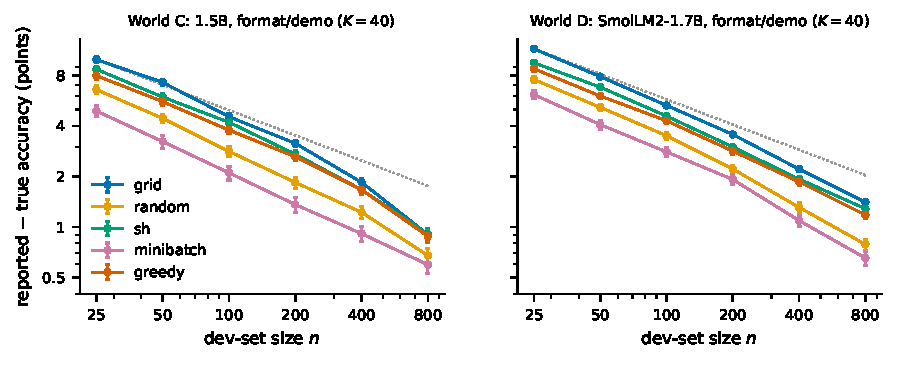
\includegraphics[width=.8\textwidth]{figs/gap_vs_n_extra.pdf}\caption{As \cref{fig:gap} for worlds C and D.}\end{figure}
\begin{table}[H]\caption{Reported $-$ true accuracy (points) by optimizer, worlds C and D.}\label{tab:gap_extra}\centering\scriptsize\setlength{\tabcolsep}{3pt}\begin{tabular}{lrrrr}\toprule
 & $n{=}50$ & 100 & 200 & 400 \\\midrule
\multicolumn{5}{l}{\emph{C: Qwen2.5-1.5B, format/demo grid ($K{=}40$)}} \\
Exhaustive & 7.3$\pm$0.3 & 4.5$\pm$0.2 & 3.1$\pm$0.1 & 1.8$\pm$0.1 \\
Random-8 & 4.4$\pm$0.3 & 2.8$\pm$0.2 & 1.8$\pm$0.1 & 1.2$\pm$0.1 \\
Succ. halving & 5.9$\pm$0.3 & 4.2$\pm$0.2 & 2.7$\pm$0.1 & 1.7$\pm$0.1 \\
Minibatch (MIPRO-like) & 3.2$\pm$0.3 & 2.1$\pm$0.2 & 1.4$\pm$0.1 & 0.9$\pm$0.1 \\
Greedy coord. & 5.6$\pm$0.3 & 3.8$\pm$0.2 & 2.6$\pm$0.1 & 1.7$\pm$0.1 \\
\multicolumn{5}{l}{\emph{D: SmolLM2-1.7B, format/demo grid ($K{=}40$)}} \\
Exhaustive & 7.9$\pm$0.2 & 5.3$\pm$0.1 & 3.6$\pm$0.1 & 2.2$\pm$0.1 \\
Random-8 & 5.2$\pm$0.2 & 3.5$\pm$0.2 & 2.2$\pm$0.1 & 1.3$\pm$0.1 \\
Succ. halving & 6.8$\pm$0.2 & 4.6$\pm$0.2 & 3.0$\pm$0.1 & 1.9$\pm$0.1 \\
Minibatch (MIPRO-like) & 4.1$\pm$0.2 & 2.8$\pm$0.2 & 1.9$\pm$0.1 & 1.1$\pm$0.1 \\
Greedy coord. & 6.0$\pm$0.2 & 4.3$\pm$0.2 & 2.8$\pm$0.1 & 1.9$\pm$0.1 \\
\bottomrule
\end{tabular}
\end{table}
\begin{table}[H]\caption{Reporting protocols, exhaustive search, $n{=}100$, worlds C and D (as \cref{tab:proto}).}\label{tab:proto_extra}\centering\scriptsize\setlength{\tabcolsep}{4pt}\begin{tabular}{lrrrr}\toprule
Protocol & bias & RMSE & coverage & width \\\midrule
\multicolumn{5}{l}{\emph{C: Qwen2.5-1.5B, format/demo grid ($K{=}40$)}} \\
Naive (dev score) & +4.5 & 6.2 & 0.85 & 18.3 \\
Holdout split (50/50) & +0.0 & 6.5 & 0.96 & 24.4 \\
5-fold cross-fit & -0.2 & 5.3 & -- & -- \\
Replay bootstrap (opt.) & +1.1 & 4.6 & -- & -- \\
Replay bootstrap (.632) & +1.4 & 4.6 & -- & -- \\
Empirical Bayes & +2.1 & 5.1 & 0.92 & 17.4 \\
Max-t simultaneous & +4.5 & 6.2 & 0.99 & 27.8 \\
Conditional (winner) & -7.1 & 16.9 & 0.77 & 25.1 \\
Ladder ($n^{-1/2}$) & +0.7 & 4.9 & -- & -- \\
\multicolumn{5}{l}{\emph{D: SmolLM2-1.7B, format/demo grid ($K{=}40$)}} \\
Naive (dev score) & +5.3 & 6.3 & 0.78 & 16.9 \\
Holdout split (50/50) & +0.2 & 5.7 & 0.95 & 21.6 \\
5-fold cross-fit & -0.1 & 4.9 & -- & -- \\
Replay bootstrap (opt.) & +1.4 & 3.9 & -- & -- \\
Replay bootstrap (.632) & +1.8 & 3.9 & -- & -- \\
Empirical Bayes & +0.8 & 3.7 & 0.97 & 16.2 \\
Max-t simultaneous & +5.3 & 6.3 & 0.99 & 26.0 \\
Conditional (winner) & -6.5 & 13.4 & 0.80 & 23.5 \\
Ladder ($n^{-1/2}$) & +1.4 & 4.2 & -- & -- \\
\bottomrule
\end{tabular}
\end{table}
\begin{table}[H]\caption{Claims, worlds C and D (as \cref{tab:concl}).}\label{tab:concl_extra}\centering\scriptsize\setlength{\tabcolsep}{2.5pt}\begin{tabular}{rrrrrrr}\toprule
$n$ & false claim & (holdout) & lift & holdout lift & A$-$B & (holdout) \\\midrule
\multicolumn{7}{l}{\emph{C: Qwen2.5-1.5B, format/demo grid ($K{=}40$)}} \\
50 & 0.25 & 0.03 & 7.0 / 0.1 & -0.4 & 3.6 / 0.2 & 0.0 \\
100 & 0.19 & 0.03 & 5.1 / 0.4 & 0.1 & 2.7 / 0.3 & 0.1 \\
200 & 0.14 & 0.02 & 3.8 / 0.7 & 0.4 & 2.0 / 0.4 & 0.2 \\
400 & 0.11 & 0.01 & 2.9 / 1.1 & 0.7 & 1.6 / 0.7 & 0.5 \\
\multicolumn{7}{l}{\emph{D: SmolLM2-1.7B, format/demo grid ($K{=}40$)}} \\
50 & 0.22 & 0.04 & 7.8 / -0.0 & -0.2 & 3.9 / 0.1 & -0.0 \\
100 & 0.18 & 0.03 & 5.6 / 0.3 & -0.0 & 2.8 / 0.3 & 0.3 \\
200 & 0.15 & 0.03 & 4.1 / 0.7 & 0.3 & 2.0 / 0.3 & 0.1 \\
400 & 0.11 & 0.02 & 3.1 / 1.0 & 0.7 & 1.6 / 0.4 & 0.3 \\
\bottomrule
\end{tabular}
\end{table}
\begin{table}[H]\caption{Sample splitting, worlds C and D (as \cref{tab:split}).}\label{tab:split_extra}\centering\scriptsize\setlength{\tabcolsep}{3pt}\begin{tabular}{lrrrrr}\toprule
Protocol & cost & bias & RMSE & cover. & width \\\midrule
\multicolumn{6}{l}{\emph{C: Qwen2.5-1.5B, format/demo grid ($K{=}40$)}} \\
no split (naive) & 0.0 & +4.5 & 6.2 & 0.85 & 18.3 \\
select on 30\% / report on 70\% & 0.80 & -0.1 & 5.5 & 0.95 & 20.8 \\
select on 50\% / report on 50\% & 0.38 & +0.0 & 6.5 & 0.96 & 24.4 \\
select on 70\% / report on 30\% & 0.18 & -0.2 & 8.4 & 0.95 & 30.8 \\
\multicolumn{6}{l}{\emph{D: SmolLM2-1.7B, format/demo grid ($K{=}40$)}} \\
no split (naive) & 0.0 & +5.3 & 6.3 & 0.78 & 16.9 \\
select on 30\% / report on 70\% & 0.62 & +0.1 & 4.7 & 0.94 & 18.3 \\
select on 50\% / report on 50\% & 0.38 & +0.2 & 5.7 & 0.95 & 21.6 \\
select on 70\% / report on 30\% & 0.15 & +0.2 & 7.6 & 0.94 & 27.4 \\
\bottomrule
\end{tabular}
\end{table}
\begin{table}[H]\caption{Uncertainty from the finite pool, worlds C and D (as \cref{tab:poolboot}).}\centering\scriptsize\setlength{\tabcolsep}{4pt}\begin{tabular}{lrrr}\toprule
world, $n$ & main design & pool-bootstrap mean & 95\% range \\\midrule
C, $n{=}50$ & 7.3 & 6.7 & 6.0--7.4 \\
C, $n{=}100$ & 4.5 & 4.4 & 3.8--5.0 \\
C, $n{=}400$ & 1.8 & 1.7 & 0.9--2.2 \\
D, $n{=}50$ & 7.9 & 7.4 & 6.6--8.1 \\
D, $n{=}100$ & 5.3 & 4.8 & 4.1--5.5 \\
D, $n{=}400$ & 2.2 & 1.7 & 1.0--2.3 \\
\bottomrule
\end{tabular}
\end{table}

\section{Compute, reproducibility and disclosures}
\label{app:repro}
\textbf{Compute actually used.} The environment provided a 4-core CPU quota (no GPU, no API). LLM scoring (fp32, 3--4 threads, sharing the quota with simulations, wall-clock from the run logs): world A (1.5B, $40\times750$ question-config pairs) $\approx$12 h; world B (0.5B) $\approx$3 h; world C (1.5B, format grid) $\approx$11 h; world D (SmolLM2-1.7B, $40\times450$) $\approx$8 h; i.e.\ about 34 h in total ($\approx$1.0--1.2 s per question-configuration pair for the 1.5B models). Simulation: about 1--1.3 h of one core per (world, 2000-episode gap experiment) plus minutes for the other experiments; synthetic sweeps $<$ 2 min. \textbf{Seeds}: pool seed 12345; demonstration-set seeds 777 (A) and 4242 (B--D); all simulations seed from an md5 hash of the setting (\texttt{exp\_main.py::seed\_of}); synthetic worlds use seeds 1, 2.
\textbf{Artifact map.} Table/figure $\to$ script: \cref{tab:worlds}, \cref{tab:gap}, \cref{tab:concl}, \cref{tab:proto}, \cref{tab:split}, \cref{tab:allopt,tab:norepl,tab:optsens} $\to$ \texttt{code/make\_tables.py} (inputs: \texttt{results/sim/*.parquet} from \texttt{code/exp\_main.py}); \cref{fig:gap,fig:effort,fig:theory,fig:concl,fig:ksweep,fig:protocols} $\to$ \texttt{code/make\_figs.py} (\cref{fig:theory}a,b from \texttt{code/exp\_synth.py}); Conditional-inference sanity check $\to$ \texttt{code/check\_cond.py}. See \texttt{README.md} for commands and expected run times.
\textbf{Negative and abandoned results.} (i) A llama.cpp CPU backend ran at $\approx$2 tokens/s here and was abandoned for torch fp32. (ii) World A turned out to be nearly flat (prompt differences of $\le$3 points, reliability $\approx 0$), which led us to add worlds B and A$\cup$B (real spread) and later C and D. (iii) The first SmolLM2 run was OOM-killed on 8-shot prompts (no grouped-query attention makes the expanded prefix cache large); we capped the cache size and resumed; world D uses 450 questions because that run was slower than planned (for $n$ near $N{=}450$ the i.i.d.\ pool design is less meaningful, so we report $n\le400$ for D). (iv) The first version of our empirical-Bayes interval (posterior sd) under-covered (0.45--0.72) and was replaced by the recentred interval of the main text; the first conditional-inference implementation mishandled exact ties (coverage 0.57--0.70) and was fixed by jittering (it still under-covers on discrete data); max-$t$ and EB for adaptive optimizers are heuristic; a trimmed-EB variant (restricting to near-winner configurations) helped only at large $n$ in A$\cup$B and was dropped. (v) We did not run DSPy/MIPRO themselves.
\textbf{Use of LLM assistance.} The research agent (an AI model) designed, ran and wrote up all of this work autonomously. \textbf{Content restrictions.} Literature was searched with scholarly-search tools only for classical statistics/ML references (winner's curse, cross-validation, post-selection inference, adaptive data analysis, prompt optimization); a search for ``optimizer's curse'' listed two 2025--2026 decision-analysis papers (policy evaluation), which were not opened. We did not intentionally search for, open or use the specific prior study the task excludes, and did not recognise any search result as such.
\textbf{Reproducibility checklist (ICML does not mandate one; provided for completeness).} Claims match results: yes (all numbers are produced by the listed scripts). Limitations: \cref{sec:discussion}. Theory assumptions/proofs: \cref{sec:setting}. Datasets, code, seeds, compute: this section and README. Error bars: 95\% CIs in tables/figures; coverage s.e.\ in captions. Statistical significance: Monte-Carlo s.e.; no hypothesis tests on the results themselves. Licenses: MMLU-Pro (MIT), Qwen2.5 (Apache-2.0 for 0.5B/1.5B). Human subjects: none.
